\graphicspath{{./figures}}

\section{Radiosonde}

The helical antenna was setup to receive the radiosonde GFSK signal using the RTL-SDR USB dongle. A resultant "squelch" signal was observed to be received in one second intervals, and the frequency domain of this signal is plotted in Figure \ref{fig:radiosondeSpectrum} using GNU Radio software.

\begin{figure}[!htb]
  \centering
  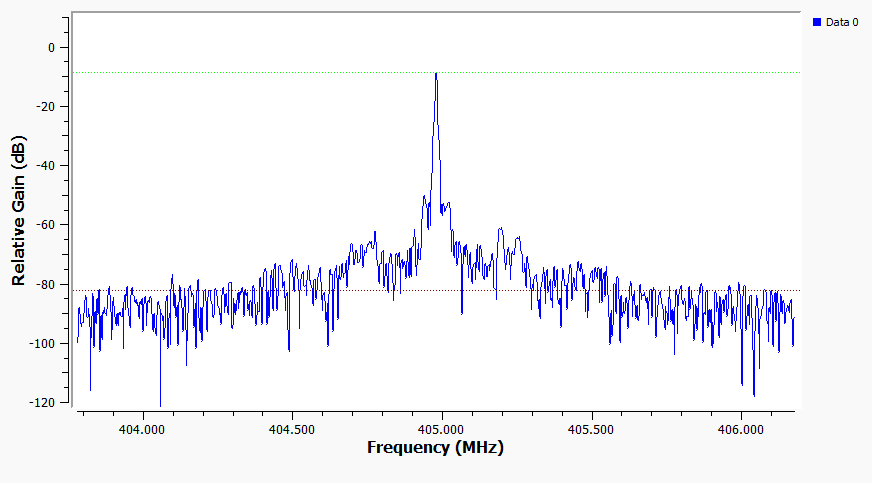
\includegraphics[width=0.8\textwidth]{radiosondeSpectrum}
  \caption{Received Radiosonde Signal FFT}
  \label{fig:radiosondeSpectrum}
\end{figure}